\begin{figure*}[t]
\centering
{\footnotesize
\textcolor[HTML]{1FDB40}{$\times$} 참조 코너\quad
\textcolor[HTML]{0089DB}{$\circ$} Base\quad
\textcolor[HTML]{DF267F}{$\diamond$} N3 (seed 1)\quad
\textcolor[HTML]{DE9600}{$\rightarrow$} 실제 이동 방향}
\par\smallskip
\begin{tabular}{@{}p{.30\textwidth}@{\hspace{.015\textwidth}}p{.23\textwidth}@{\hspace{.025\textwidth}}p{.39\textwidth}@{}}
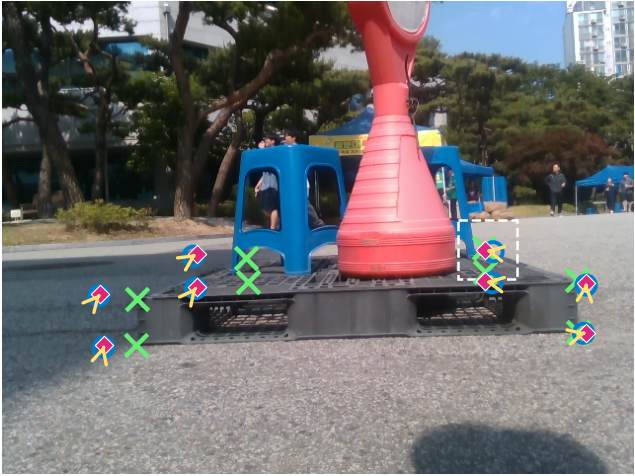
\includegraphics[width=\linewidth]{figures/example_1_frame.png} &
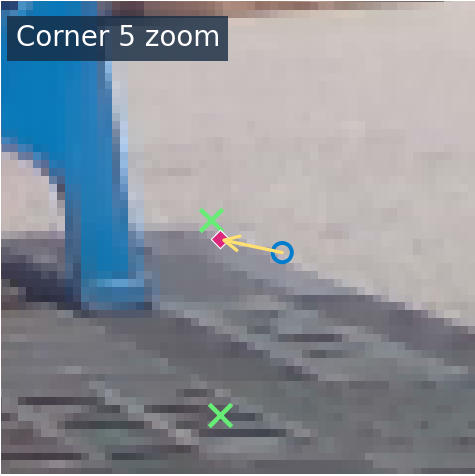
\includegraphics[width=\linewidth]{figures/example_1_zoom.png} &
\begin{minipage}[b]{\linewidth}\footnotesize
\textbf{(a) 큰 오류의 부분 감소}\\
직사각형 플라스틱, $(1.10,1.30,0.11)$m\\
Base 27.21px $\rightarrow$ N3 25.42px\\
코너 5 확대; 최대 코너 이동 8.00px\\
\texttt{eval\_pallet07}\\
프레임 \texttt{1778652125245035520}
\end{minipage}\\[4pt]
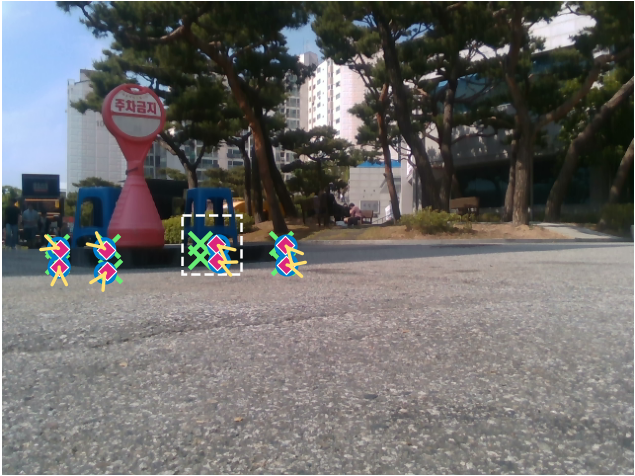
\includegraphics[width=\linewidth]{figures/example_2_frame.png} &
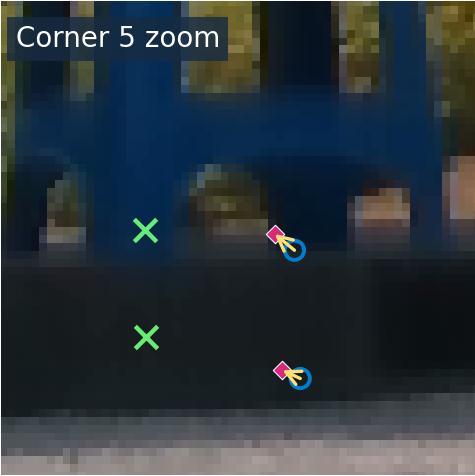
\includegraphics[width=\linewidth]{figures/example_2_zoom.png} &
\begin{minipage}[b]{\linewidth}\footnotesize
\textbf{(b) 코너 오차 감소}\\
직사각형 플라스틱, $(1.10,1.30,0.11)$m\\
Base 8.48px $\rightarrow$ N3 7.45px\\
코너 5 확대; 최대 코너 이동 3.26px\\
\texttt{eval\_pallet09}\\
프레임 \texttt{1778653706706429696}
\end{minipage}\\[4pt]
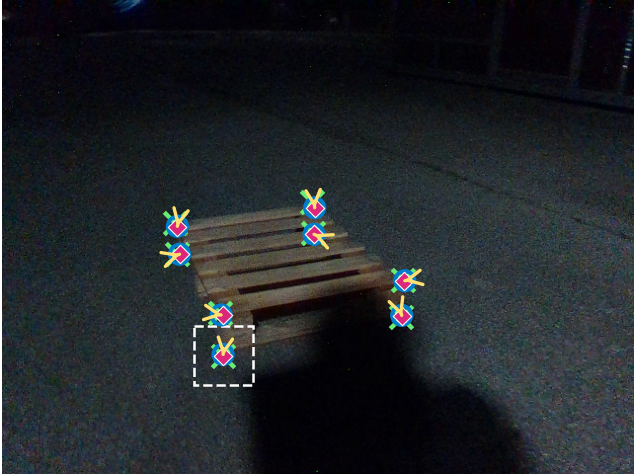
\includegraphics[width=\linewidth]{figures/example_3_frame.png} &
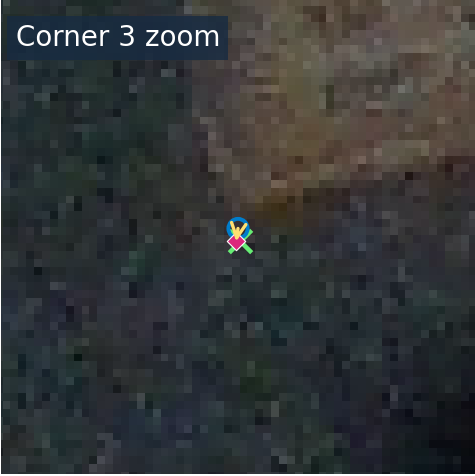
\includegraphics[width=\linewidth]{figures/example_3_zoom.png} &
\begin{minipage}[b]{\linewidth}\footnotesize
\textbf{(c) 원래 양호한 예측의 소폭 악화}\\
직사각형 목재, $(0.80,0.59,0.14)$m\\
Base 2.90px $\rightarrow$ N3 2.99px\\
코너 3 확대; 최대 코너 이동 1.66px\\
\texttt{wood\_night\_01}, 프레임 \texttt{029919}
\end{minipage}
\end{tabular}
\caption{동일한 기존 영상·좌표의 보정 예시. 그림은 고정 seed 1을 표시하고, 사례 선정에는 세 seed의 영상별 평균 코너 오차 변화가 사용되었다. 수치는 알려진 코너 0--7의 대칭 고려 영상별 평균으로 주표의 풀링 중앙값과 다르다. 원래 예시의 영상과 확대 영역을 자르고 설명 레이블만 재배치했으며 코너 위치를 변경하지 않았다. 큰 오류의 부분 감소와 소폭 악화를 함께 보존한다.}\label{fig:examples}
\end{figure*}
